% chktex-file 44
%%%%%%%%%%%%%%%%%%%%%%%%%%%%% The Light Curve of \groj %%%%%%%%%%%%%%%%%%%%
\chapter{The Light Curve of \groj}\label{cha:lightcurve}

The initial step in calculating the mass of the black hole in \groj\ is to measure the ellipsoidal variability of the system. Here we explain how we obtained the light curve of \groj\ from our observations. %

%%%%%%%%%%%%%%%%%%%%%%%%%%%%% Photometry of \groj %%%%%%%%%%%%%%%%%%%%

\section{Photometry of \groj}\label{cha:lightcurve:sec:Photometry}

For the CTIO and KECK $J$-- and $K$--band observations, we performed the following procedure to produce light curves for each period of observation. %

%%%%%%%%%%%%%%%%%%%%%%%%%%%%% Initial Data Reduction %%%%%%%%%%%%%%%%%%%%

\subsection{The Initial Data Reduction}\label{cha:lightcurve:sec:Photometry:subsec:InitialDataReduction}

First, the images were background subtracted, as discussed in \S~\ref{cha:InfraredDataReductionTechniques:sec:Photometry:subsec:BackgroundSubtraction}%
, to remove the high background typical of infrared images.%

\vspace{\myparskip}

Second, a \textbf{dome flat} was produced for the 1998 CTIO data, and the alternative method of \textbf{median combination} was employed to create a flatfield for the 1995 CTIO images (see \S~\ref{cha:InfraredDataReductionTechniques:sec:Photometry:subsec:Flatfield}). However, dome flats were not obtained for the KECK images of \groj: since the
total number of raw images obtained using the KECK telescope was too
small for an accurate flatfield to be produced (using the median combination technique), the KECK images were
not divided by any flatfield. %

\vspace{\myparskip}

Third, a bad pixel map was produced in the manner described in \S~\ref{cha:InfraredDataReductionTechniques:sec:Photometry:subsec:BadPixels} for the 1998 and 1995 data sets. Due to the small number of KECK images, no bad pixel map was created
for the KECK data. However, a visual inspection of the KECK images
determined that no bad pixels were present near the target stars. %

\vspace{\myparskip}

%%%%%%%%%%%%%%%%%%%%%%%%%%%%% ctio95_g001_3 %%%%%%%%%%%%%%%%%%%%
\begin{figure}[!htb]
\begin{center}
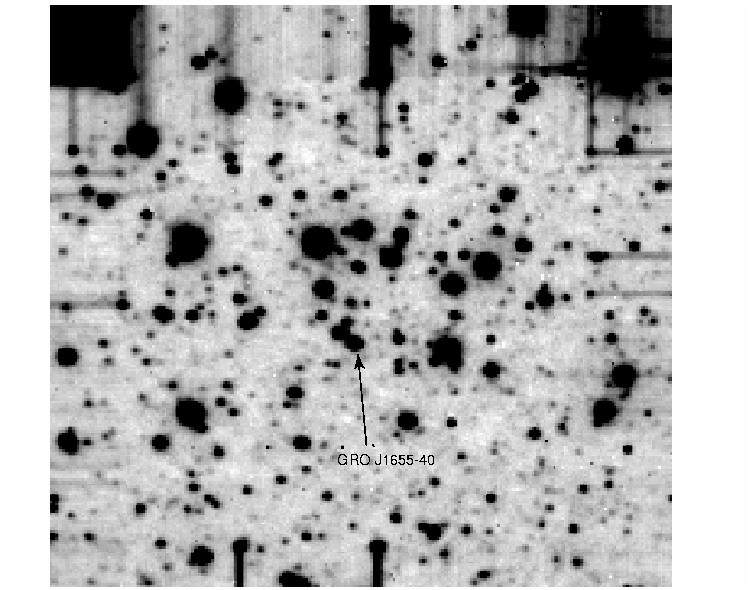
\includegraphics[width=5.0in]{ctio95_g001_3}
\caption{%
Example of an average combined grid of frames, with our system of interest
(\mbox{\groj}) indicated. This 15 second exposure, which has a
field of view of $\sim 166\arcsec \times 166\arcsec $, was
obtained using the CTIO CIRIM detector during June 1995.}\label{cha:lightcurve:sec:Photometry:subsec:CombiningTheGrid:fig:ctio95_g001_3}
\end{center}
\end{figure}
%%%%%%%%%%%%%%%%%%%%%%%%%%%%%%%%%%%%%%%%%%%%%%%%%%%%%%%%%%%%%%%%%%

Finally, each grid of images were combined to produce processed images of our target system (see \S~\vref{cha:InfraredDataReductionTechniques:sec:Photometry:subsec:CombiningTheGrid} for details). Figure~%
\vref{cha:lightcurve:sec:Photometry:subsec:CombiningTheGrid:fig:ctio95_g001_3}%
\ is an example of a combined grid from the 1995 $K_s$--band data set. %


%%%%%%%%%%%%%%%%%%%%%%%%%%%%% Relative Photometry %%%%%%%%%%%%%%%%%%%%

\subsection{Calculating the Relative Magnitudes}\label{cha:lightcurve:sec:Photometry:subsec:RelativePhotometry}

%%%%%%%%%%%%%%%%%%%%% 1648_1656_3 %%%%%%%%%%%%%%%%%%%%
\begin{figure}[!htb]
\begin{center}
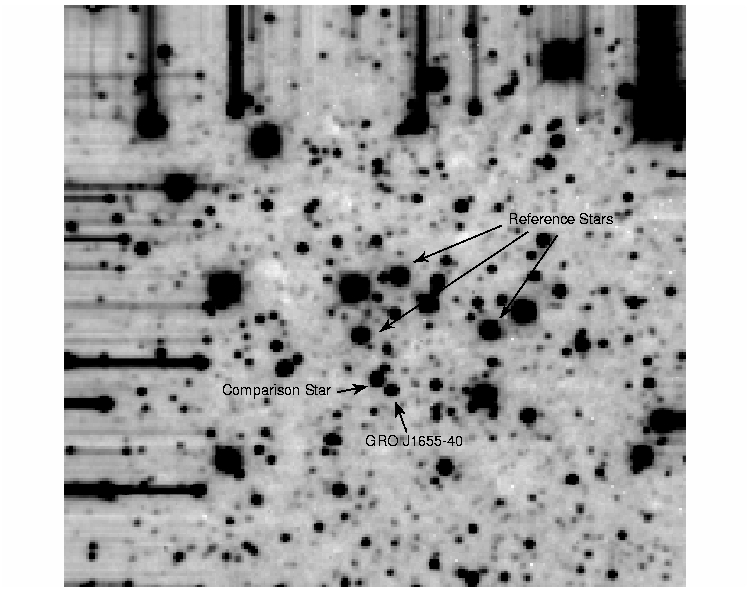
\includegraphics[width=5.0in]{1648_1656_3}
\caption{%
Field of view for the 1998 $K_s$ data, indicating the target,
comparison and reference stars. This $\sim 166\arcsec \times
166\arcsec$ image was obtained with a 30 second exposure using the
CTIO CIRIM detector during June 1998. }\label{cha:lightcurve:sec:Photometry:subsec:RelativePhotometry:fig:1648_1656_3}
\end{center}
\end{figure}
%%%%%%%%%%%%%%%%%%%%%%%%%%%%%%%%%%%%%%%%%%%%%%%%%%%%%%%%%%%%%%%%%%

Once the raw images were processed, we proceeded to run \texttt{DAOPHOT} to measure the magnitudes of \groj\ and a comparison star relative to several reference stars in the same field of view. The procedure outlined in \S~\ref{cha:InfraredDataReductionTechniques:sec:Photometry:subsec:RelativePhotometry} was  used for each period of observation and each filter. The stars chosen are given in Figure~%
\vref{cha:lightcurve:sec:Photometry:subsec:RelativePhotometry:fig:1648_1656_3}%
. %

%%%%%%%%%%%%%%%%%%%%%%%%%%%%% kctio98prefolded %%%%%%%%%%%%%%%%%%%%
\begin{figure}[!htb]
\begin{center}
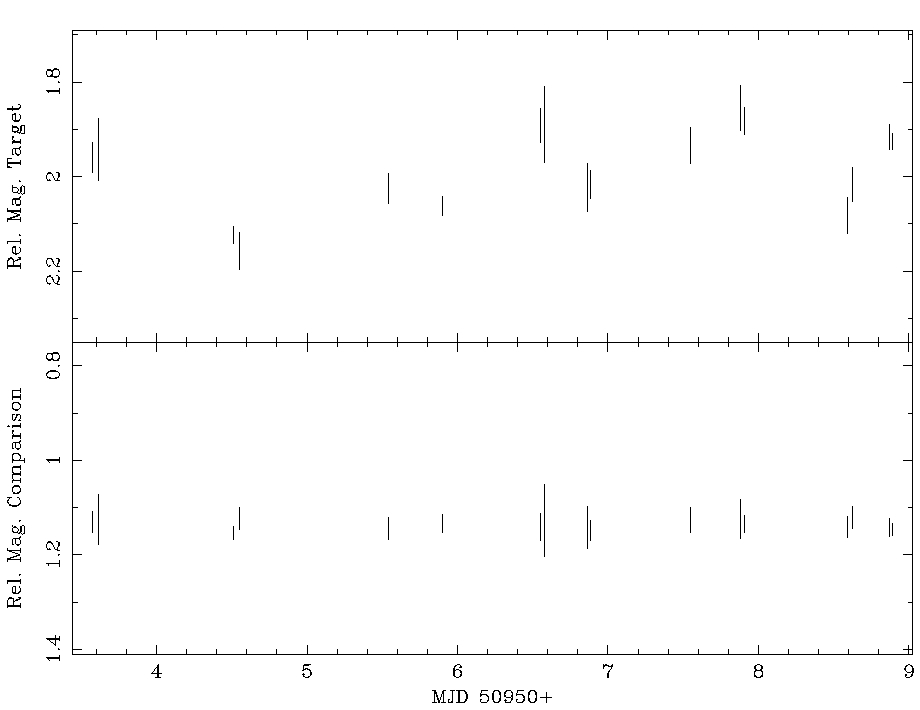
\includegraphics[width=5.0in]{kctio98prefolded}
\caption{%
Plot of relative magnitudes of target star \groj\ and comparison star
for the 1998 $K_s$ observations. %
}\label{cha:lightcurve:sec:Photometry:subsec:RelativePhotometry:fig:kctio98prefolded}
\end{center}
\end{figure}
%%%%%%%%%%%%%%%%%%%%%%%%%%%%%%%%%%%%%%%%%%%%%%%%%%%%%%%%%%%%%%%%%%

\vspace{\myparskip}

We then plotted the two relative magnitudes against the Julian
Dates of the observations to obtain the light curves of the target and
comparison star (see Figure~%
\ref{cha:lightcurve:sec:Photometry:subsec:RelativePhotometry:fig:kctio98prefolded}%
). Since the relative magnitude of the comparison star was constant over this period of observation, we assumed that the variability in the relative magnitude of \groj\ was due to the changing magnitude of the system itself. %

\vspace{\myparskip}

Finally, using the orbital
ephemeris determined by Van~der~Hooft et~al.\ %
\citeyear{VanDerHooft_et_al.:1998}%
\ (see \S~%
\vref{cha:GROJ1655-40:sec:IntroductionToJ1655:subsec:PropertiesOfJ1655:subsubsec:SystemProperties:eqn:Ephemeris}%
),%
\ we folded\footnote{\label{cha:lightcurve:sec:Photometry:subsec:RelativePhotometry:foot:MJD}%
When folding the data, the Heliocentric Julian Date (HJD) of the
observation was taken to be equal to the Julian Date (JD) of
observation. Although this introduced an error of 8 minutes, this is
small compared to the error in the orbital period ($2\fd62168\pm0\fd00014$:
van~der~Hooft et~al.\ %
\citeyearNP{VanDerHooft_et_al.:1998}%
).}%
\ the light curve of \groj\ on the orbital period. We then introduced
an offset to the 1998 $K_s$ data to move one of the points to phase
0.5, and so align the minima and maxima with the appropriate
phases. This offset was within the error of 3\% incurred by
extrapolating the ephemeris to the time of observation. %

%%%%%%%%%%%%%%%%%%%%%%%%%%%%% kctio95plot %%%%%%%%%%%%%%%%%%%%
\begin{figure}[!htb]
\begin{center}
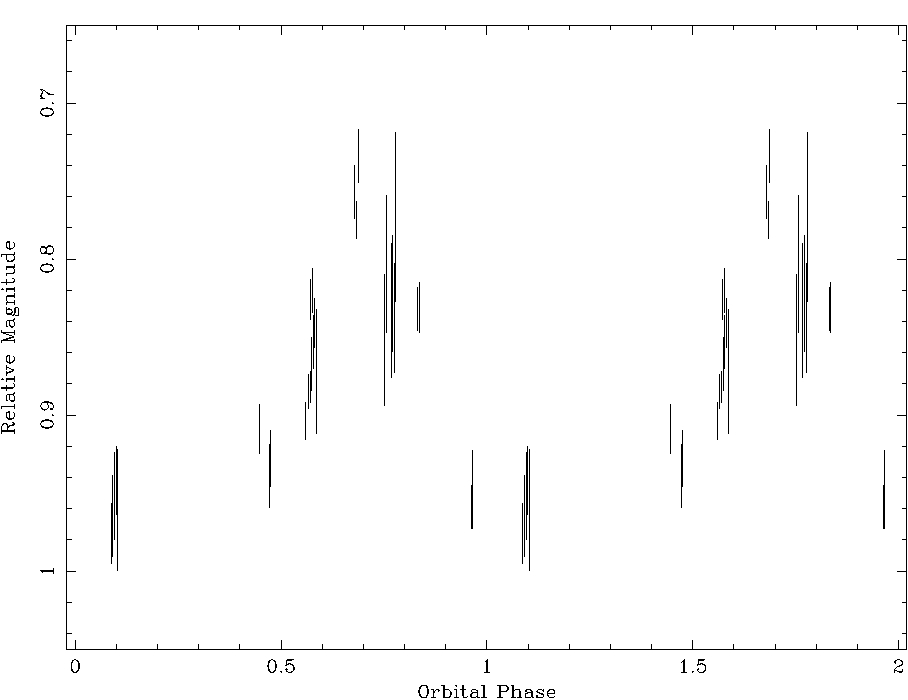
\includegraphics[width=5.0in]{kctio95plot}
\caption{%
The light curve of \groj\ during June 1995.
The fold is repeated for clarity. %
}\label{cha:lightcurve:sec:Photometry:subsec:RelativePhotometry:fig:kctio95plot}
\end{center}
\end{figure}
%%%%%%%%%%%%%%%%%%%%%%%%%%%%%%%%%%%%%%%%%%%%%%%%%%%%%%%%%%%%%%%%%%

\vspace{\myparskip}

Figure~%
\ref{cha:lightcurve:sec:Photometry:subsec:RelativePhotometry:fig:kctio95plot}%
\ and Figure~%
\ref{cha:lightcurve:sec:Photometry:subsec:RelativePhotometry:fig:kctio98plot}%
\ show the folded $K_s$ light curves for each year. As can be seen from Figure~%
\ref{cha:lightcurve:sec:Photometry:subsec:RelativePhotometry:fig:kctio98plot},%
\ an ellipsoidal variability was apparent from the 1998 $K_s$ light curve. %

%%%%%%%%%%%%%%%%%%%%%%%%%%%%% kctio98plot %%%%%%%%%%%%%%%%%%%%
\begin{figure}[!htb]
\begin{center}
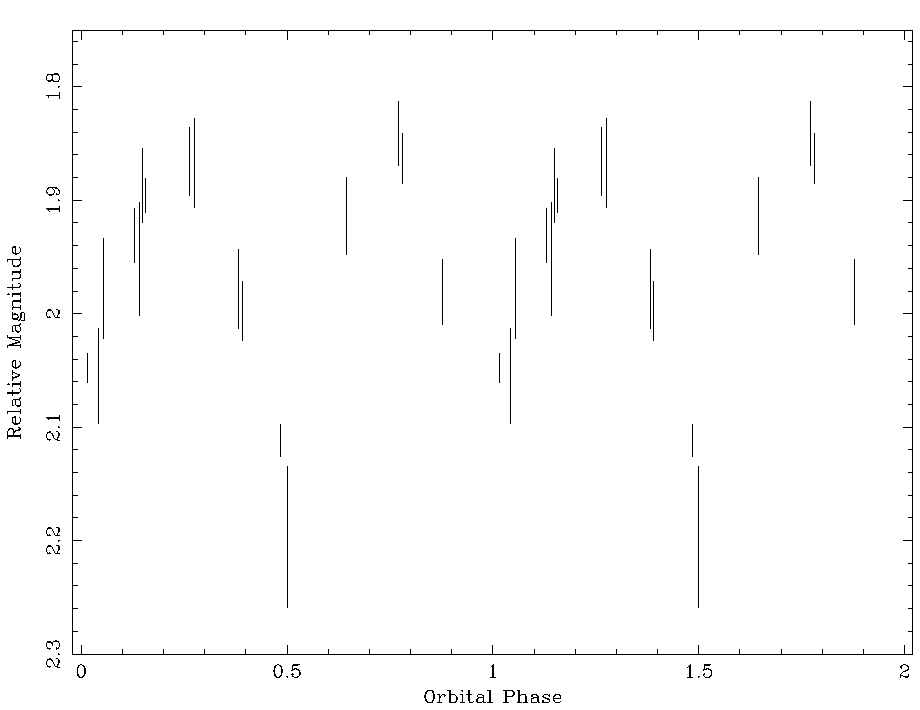
\includegraphics[width=5.0in]{kctio98plot}
\caption{%
The ellipsoidal variability of \groj\ during May-June 1998. %
}\label{cha:lightcurve:sec:Photometry:subsec:RelativePhotometry:fig:kctio98plot}
\end{center}
\end{figure}
%%%%%%%%%%%%%%%%%%%%%%%%%%%%%%%%%%%%%%%%%%%%%%%%%%%%%%%%%%%%%%%%%%

\vspace{\myparskip}

Using the folded light curves, we then calculated the phase averaged relative magnitudes of \groj\ (see \S~\ref{cha:InfraredDataReductionTechniques:sec:Photometry:subsec:RelativePhotometry:topic:parm}). Since the 1995 $J$--band data consisted of only one combined image, it was not
possible to get the phase average relative magnitude of \groj. The
relative magnitude of \groj\ in the single image was taken as the
average. Table~%
\vref{cha:lightcurve:sec:Photometry:subsec:RelativePhotometry:tab:phasemag}
lists the averaged magnitudes calculated.

\begin{table}[htb]
\caption{\groj\ Phase Averaged Relative Magnitudes}\label{cha:lightcurve:sec:Photometry:subsec:RelativePhotometry:tab:phasemag}

\begin{minipage}{\linewidth}
\renewcommand{\thefootnote}{\thempfootnote}

\begin{center}
\begin{tabular}{|l||||c|c|}

\hline
Year & $J$ Relative Magnitude (mag) & $K_s$ Relative Magnitude (mag) \\\hline\hline\hline\hline
1995 & $0.01\pm0.05$ & $0.68\pm0.05$ \\\hline
1998 & $1.00\pm0.05$ & $1.71\pm0.05$ \\\hline
\hline
\end{tabular}
\end{center}
\end{minipage}
\end{table}

%%%%%%%%%%%%%%%%%%%%%%%%%%%%% Apparent Magnitudes %%%%%%%%%%%%%%%%%%%%

\subsection{Obtaining the Apparent Magnitudes}\label{cha:lightcurve:sec:Photometry:subsec:PhotometricCalibration}

We next calculated the apparent magnitude of the system. We did this by photometrically calibrating our data. (See \S~\vref{cha:InfraredDataReductionTechniques:sec:Photometry:subsec:AperturePhotometry} for more details.) %

%%%%%%%%%%%%%%%%%%%%%%%%%%%%% CTIO CIRIM Images %%%%%%%%%%%%%%%%%%%%

\subsubsection{CTIO CIRIM Images}\label{cha:lightcurve:sec:Photometry:subsec:PhotometricCalibration:subsubsec:ctio}

We first attempted to calibrate the images using the observations made
with the CTIO CIRIM detector. Previously \citeN{Curran:2001} calculated the number of counts per second for a star of 10th magnitude ($f_{10}$) for the CTIO CIRIM detected. These values were:%
\begin{eqnarray} \label{cha:lightcurve:sec:Photometry:subsec:PhotometricCalibration:subsubsec:ctio:eqn:f10}
f_{10}(J) = 10,900\pm400\,\mathrm{counts/sec},\\\nonumber% chktex 35
f_{10}(K_s) = 6580\pm80\,\mathrm{counts/sec}.% chktex 35
\end{eqnarray} %

%%%%%%%%%%%%%%%%%%%%%%%%%%%%% 1648_1656_ctio_2 %%%%%%%%%%%%%%%%%%%%
\begin{figure}[!htb]
\begin{center}
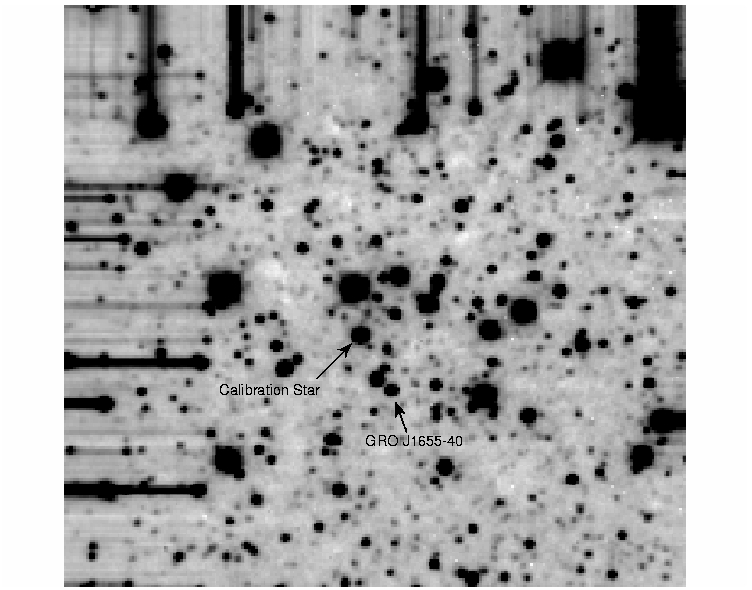
\includegraphics[width=5.0in]{1648_1656_ctio_2}
\caption{%
The selected photometric image from the 1998 $K_s$ data, with the
target star and calibration star indicated. This 30 second exposure,
with a field of view of $\sim 166\arcsec \times 166\arcsec $, was
obtained using the CTIO CIRIM detector during June 1998. }\label{cha:lightcurve:sec:Photometry:subsec:PhotometricCalibration:subsubsec:ctio:fig:1648_1656_ctio_2}
\end{center}
\end{figure}
%%%%%%%%%%%%%%%%%%%%%%%%%%%%%%%%%%%%%%%%%%%%%%%%%%%%%%%%%%%%%%%%%%

\vspace{\myparskip}

The log of the 1998 observations was consulted to determine
which of the original images were taken during photometric
conditions. One grid of such images was selected and aperture
photometry was performed on the combined image of this grid. The chosen image is shown in Figure~%
\vref{cha:lightcurve:sec:Photometry:subsec:PhotometricCalibration:subsubsec:ctio:fig:1648_1656_ctio_2}%
, and the calibration star is marked. %

\vspace{\myparskip}

\begin{table}[htb]
\caption{Apparent Magnitude of Calibration Star}\label{cha:lightcurve:sec:Photometry:subsec:PhotometricCalibration:subsubsec:ctio:tab:calibappmag}

\begin{minipage}{\linewidth}
\renewcommand{\thefootnote}{\thempfootnote}

\begin{center}
\begin{tabular}{|c|c|}

\hline
$J$ Apparent Magnitude (mag) & $K_s$ Apparent Magnitude (mag)\\\hline\hline\hline\hline
$12.81\pm0.05$ & $11.29\pm0.05$ \\\hline
\hline
\end{tabular}
\end{center}
\end{minipage}
\end{table}

The magnitudes of the comparison star in each filter are given in Table~%
\ref{cha:lightcurve:sec:Photometry:subsec:PhotometricCalibration:subsubsec:ctio:tab:calibappmag}%
.

\vspace{\myparskip}

\begin{table}[htb]
\caption{Initial \groj\ Apparent Magnitudes}\label{cha:lightcurve:sec:Photometry:subsec:PhotometricCalibration:subsubsec:ctio:tab:initappmag}

\begin{minipage}{\linewidth}
\renewcommand{\thefootnote}{\thempfootnote}

\begin{center}
\begin{tabular}{|l||||c|c|}

\hline
Year & $J$ Apparent Magnitude (mag) & $K_s$ Apparent Magnitude (mag)\\\hline\hline\hline\hline
1995 & $12.71\pm0.05$ & $11.98\pm0.05$ \\\hline
1998 & $13.81\pm0.05$ & $13.00\pm0.05$ \\\hline
\hline
\end{tabular}
\end{center}
\end{minipage}
\end{table}

Using these calibration magnitudes, the $K_s$--band and $J$--band magnitude of \groj\ were calculated as described in \S~\ref{cha:InfraredDataReductionTechniques:sec:Photometry:subsec:AperturePhotometry}. These values are listed in Table~%
\vref{cha:lightcurve:sec:Photometry:subsec:PhotometricCalibration:subsubsec:ctio:tab:initappmag}. The magnitudes calculated from the 1998 data were taken as the quiescent magnitudes of \groj, whereas the 1995 magnitudes were taken to be outburst magnitudes (see \S~\ref{cha:GROJ1655-40:sec:ObservationsOfJ1655:subsec:DetailsOfTheObservations}). It can be immediately seen that the system was brighter during outburst by approximately one magnitude. %


%%%%%%%%%%%%%%%%%%%%%%%%%%%%% KECK SCAM Images %%%%%%%%%%%%%%%%%%%%

\subsubsection{KECK SCAM Images}\label{cha:lightcurve:sec:Photometry:subsec:PhotometricCalibration:subsubsec:keck}

The second calibration was performed using the KECK observations of \\%
% WHITE SPACE %
\groj. Although these observations were not made under ideal photometric conditions, it was hoped that these images would provide a check for the earlier calibration. %

%%%%%%%%%%%%%%%%%%%%%%%%%%%%% keck00_2 %%%%%%%%%%%%%%%%%%%%
\begin{figure}[!htb]
\begin{center}
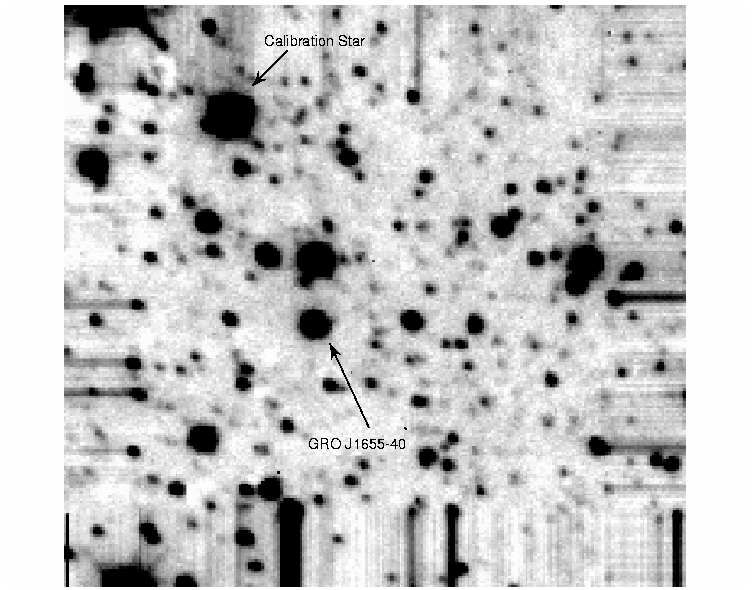
\includegraphics[width=5.0in]{keck00_2}
\caption{%
The field of view for the KECK images. The target star and the
calibration star are marked. This $\sim 46\arcsec \times 46\arcsec$
image was obtained with a $1\times10$ second exposure using the KECK
S-CAM detector during June 1998. }\label{cha:lightcurve:sec:Photometry:subsec:PhotometricCalibration:subsubsec:keck:fig:keck00_2}
\end{center}
\end{figure}
%%%%%%%%%%%%%%%%%%%%%%%%%%%%%%%%%%%%%%%%%%%%%%%%%%%%%%%%%%%%%%%%%%

\vspace{\myparskip}

During a KECK SCAM observation run prior to our run in 2000, the value of
$f_{10}$ was determined to be approximately 400,000 counts per second~\cite{Callanan:2001}%
. We applied aperture photometry to the calibration star in the
KECK images to measure the count rate $f$ of this star. Figure~%
\vref{cha:lightcurve:sec:Photometry:subsec:PhotometricCalibration:subsubsec:keck:fig:keck00_2}%
\ shows the processed KECK image with the calibration star
indicated. The apparent $K$--band magnitude, $K$, of the star was then
determined to be $11.25\pm0.05$\,mag. The apparent $K$ magnitude of \groj\ was then calculated, and found to be $12.95\pm0.05$\,mag. This value was consistent with the
preceding measurement using the 1998 CTIO images%
\footnote{\label{cha:lightcurve:sec:Photometry:subsec:PhotometricCalibration:foot:kks}
We take the magnitude of the star in the $K$-- and $K_s$--bands to be
equal.
}, validating the calibration. %

%%%%%%%%%%%%%%%%%%%%%%%%%%%%% 2MASS All-Sky Point Source Catalog %%%%%%%%%%%%%%%%%%%%

\subsubsection{2MASS All-Sky Point Source Catalog}\label{cha:lightcurve:sec:Photometry:subsec:PhotometricCalibration:subsubsec:2mass}

During the preparation of this thesis, the \textbf{All-Sky Point Source Catalog (PSC)} from the \textbf{Two Micron All Sky Survey (2MASS)}%
\footnote{\label{cha:lightcurve:sec:Photometry:subsec:PhotometricCalibration:subsubsec:2mass:foot:PSC}
\url{http://irsa.ipac.caltech.edu/}
}%
\ was released. We decided to verify our calibration of \groj\ using this more reliable source. %

\vspace{\myparskip}

\begin{table}[htb]
\caption{2MASS Apparent Magnitudes}\label{cha:lightcurve:sec:Photometry:subsec:PhotometricCalibration:subsubsec:2mass:tab:2massmags}

\begin{minipage}{\linewidth}
\renewcommand{\thefootnote}{\thempfootnote}

\DeclareFixedFootnote{\phase}{At Phase 0.21.} % For fixed footnote

\begin{center}
\begin{tabular}{|l||||c|c|}

\hline
Source & $J$ Apparent Magnitude (mag) & $K_s$ Apparent Magnitude (mag)\\\hline\hline\hline\hline
\groj\ \phase\ & $13.516\pm0.029$ & $12.744\pm0.034$ \\\hline
Calibration Star & $12.757\pm0.029$ & $11.153\pm0.021$ \\\hline
\hline
\end{tabular}
\end{center}
\end{minipage}
\end{table}

First, we obtained the apparent magnitudes of both our calibration star and \groj\ from the PSC --- see Table~%
\vref{cha:lightcurve:sec:Photometry:subsec:PhotometricCalibration:subsubsec:2mass:tab:2massmags}%
\ for these values. (We noted that the Modified Julian Date of the 2MASS observation of \groj\ was $51309.7443$, which corresponds to an orbital phase of approximately $0.21$.) %

\vspace{\myparskip}

\begin{table}[htb]
\caption{\groj\ Apparent Magnitudes}\label{cha:lightcurve:sec:Photometry:subsec:PhotometricCalibration:subsubsec:2mass:tab:appmag}

\begin{minipage}{\linewidth}
\renewcommand{\thefootnote}{\thempfootnote}

\begin{center}
\begin{tabular}{|l||||c|c|}

\hline
Year & $J$ Apparent Magnitude (mag) & $K_s$ Apparent Magnitude (mag)\\\hline\hline\hline\hline
1995 & $12.77\pm0.03$ & $11.83\pm0.04$ \\\hline
1998 & $13.76\pm0.03$ & $12.86\pm0.02$ \\\hline
\hline
\end{tabular}
\end{center}
\end{minipage}
\end{table}

\vspace{\myparskip}

As there was a slight discrepancy between our CTIO measurement of our calibration star and the values from 2MASS, we decided to assume the 2MASS magnitudes for the calibration star, due to the extra reliability of this source. We then used these values to calculate the apparent magnitude of \groj\ in both the $J$-- and $K_{s}$--bands. These magnitudes are listed in Table~%
\vref{cha:lightcurve:sec:Photometry:subsec:PhotometricCalibration:subsubsec:2mass:tab:appmag}. %

\begin{table}[htb]
\caption{Apparent Magnitude of \groj}\label{cha:lightcurve:sec:Photometry:subsec:PhotometricCalibration:tab:BeerGreeneMags}

\begin{minipage}{\linewidth}
\renewcommand{\thefootnote}{\thempfootnote}

\begin{center}
\begin{tabular}{|l||||c|c|}

\hline
Source & $J$ (mag) & $K$ (mag)\\\hline\hline\hline\hline
Our 1998 $K_{s}$--band Data & $13.76\pm0.03$ & $12.86\pm0.02$ \\\hline \citeN{GreeneBailynOrosz:2001} & $13.85\pm0.02$ & $13.25\pm0.02$ \\\hline
\citeN{BeerPodsiadlowski:2001} (predicted) & 13.8 & 13.0 \\\hline
\hline
\end{tabular}
\end{center}
\end{minipage}
\end{table}

\vspace{\myparskip}

Our values for the apparent magnitude of \groj\ during quiescence were
then compared to prior estimates, listed in Table~%
\vref{cha:lightcurve:sec:Photometry:subsec:PhotometricCalibration:tab:BeerGreeneMags}%
. Although our $J$--band value coincides with the two other values,
there is a 0.4 magnitude disagreement between our $K$--band value and
that of %
\citeN{GreeneBailynOrosz:2001}%
. A similar discrepancy has already been noted by %
\citeN{BeerPodsiadlowski:2001}%
, who obtained a theoretical magnitude in better agreement with our own. This suggests our result is valid, although why the discrepancy between \citeN{GreeneBailynOrosz:2001} and ourselves exists is unclear.

%%%%%%%%%%%%%%%%%%%%%%%%%%%%% Dereddened Magnitudes %%%%%%%%%%%%%%%%%%%%

\subsection{The Dereddened Magnitudes}\label{cha:lightcurve:sec:Photometry:subsec:DereddenedMagnitude}

We then corrected this magnitude to account for interstellar extinction. We obtained a value for the reddening, $E_{B-V}$, for \groj\ from Hynes et~al.\ %
\citeyear{Hynes_et_al.:1998}: %
\begin{eqnarray} \label{cha:lightcurve:sec:Photometry:subsec:DereddenedMagnitude:eqn:EBV}
E_{B-V} = 1.2\pm0.1 \ \mathrm{mag}.
\end{eqnarray}
We derived the $K$-- and $J$--band extinction following the discussion on page~%
\pageref{cha:InfraredDataReductionTechniques:sec:Photometry:subsec:DereddenedMagnitude:eqn:CardelliAK},%
\ and obtained the values of $A_{K} = 0.42\pm0.04$\,mag and $A_{J} = 1.05\pm0.09$\,mag. (Note that the values for interstellar extinction in the infrared is much lower than that in the optical, which is given by $A_{V} = 1.3\times3.1=4.0\pm0.3$\,mag. This is as expected --- see \S~\vref{cha:InfraredDataReductionTechniques:sec:InfraredAstronomy:subsubsec:InterstellarExtinction}.) The \textbf{dereddened magnitudes} %
of \groj\ in the $J$-- and $K$--band were then calculated, and are summarised in Table~%
\vref{cha:lightcurve:sec:Photometry:subsec:DereddenedMagnitude:tab:Dered}.
The difference of 1\,mag between both the two values for $K_0$ and those
for $J_0$ were attributed to the contribution from the disk during
the outburst in 1995. %

\begin{table}[htb]
\caption{Dereddened $J$, $K$ and $J-K$ Magnitudes for 1995 and 1998}\label{cha:lightcurve:sec:Photometry:subsec:DereddenedMagnitude:tab:Dered}

\begin{minipage}{\linewidth}
\renewcommand{\thefootnote}{\thempfootnote}

\begin{center}
\begin{tabular}{|l||||c|c|c|}

\hline
Year & $J_0$ (mag)& $K_0$ (mag)& $J_{0}-K_{0}$ (mag) \\\hline\hline\hline\hline
1995 & $11.72\pm0.09$ & $11.41\pm0.06$ & $0.3\pm0.1$ \\\hline
1998 & $12.71\pm0.09$ & $12.44\pm0.04$ & $0.3\pm0.1$ \\\hline
\hline
\end{tabular}
\end{center}
\end{minipage}
\end{table}

\vspace{\myparskip}

Using the derived values of $K_0$ and $J_0$, we calculated the
dereddened \mbox{$J-K$} colour of \groj\ for 1995 and 1998. These values are also given in Table~%
\ref{cha:lightcurve:sec:Photometry:subsec:DereddenedMagnitude:tab:Dered}%
.

\vspace{\myparskip}

\begin{table}[htb]
\caption{Comparison Dereddened Magnitudes}\label{cha:lightcurve:sec:Photometry:subsec:DereddenedMagnitude:tab:BeerGreeneDeredMag}

\begin{minipage}{\linewidth}
\renewcommand{\thefootnote}{\thempfootnote}

\DeclareFixedFootnote{\pred}{From their predicted apparent magnitudes.} % For fixed footnote

\begin{center}
\begin{tabular}{|l||||c|c|c|}

\hline
Source & $J_0$ (mag)& $K_0$ (mag)& $J_{0}-K_{0}$ (mag) \\\hline\hline\hline\hline
\citeN{GreeneBailynOrosz:2001} & $12.80\pm0.09$ & $12.83\pm0.04$ & $0.0\pm0.1$ \\\hline
\citeN{BeerPodsiadlowski:2001}\pred\ & 12.75 & 12.58 & 0.17 \\\hline
\hline
\end{tabular}
\end{center}
\end{minipage}
\end{table}

Finally, we calculated the dereddened magnitudes using the apparent magnitudes calculated by %
\citeN{GreeneBailynOrosz:2001}%
\ and those predicted by %
\citeN{BeerPodsiadlowski:2001}%
. Table~%
\ref{cha:lightcurve:sec:Photometry:subsec:DereddenedMagnitude:tab:BeerGreeneDeredMag}%
\ lists these values. Again, our value for $J_{0}-K_{0}$ during quiescence
is in good agreement with that predicted by %
\citeN{BeerPodsiadlowski:2001}%
, but differs from that of %
\citeN{GreeneBailynOrosz:2001}%
. It should however be noted that in general $J_{0}-K_{0}>0$, which
supports our earlier conclusion that the $K$ magnitude derived by %
\citeN{GreeneBailynOrosz:2001}%
\ may be erroneous. %

\vspace{\myparskip}

According to %
\citeN{BeerPodsiadlowski:2001}%
, the spectral type of \groj\ lies within the range F5--G0 III-IV.\@\ We
compared our dereddened $J-K$ with that of UKIRT standard stars with a
spectral type similar to \groj. We found that the value
$J_{0}-K_{0}=0.3$\,mag was consistent with a spectral type of F0--G2
III-IV, which is in agreement with, if not as precise as, the spectral range of \citeN{BeerPodsiadlowski:2001}. %


%%%%%%%%%%%%%%%%%%%%%%%%%%%%% Absolute Magnitude %%%%%%%%%%%%%%%%%%%%

\subsection{The Absolute Magnitudes}\label{cha:lightcurve:sec:Photometry:subsec:AbsoluteMagnitude}

As a final check for self-consistency in our derived value for the magnitude of \groj, we calculated the absolute $J$-- and $K$--magnitudes of this system using Equations~%
\ref{cha:InfraredDataReductionTechniques:sec:MagnitudeScale:subsec:AbsoluteMagnitude:eqn:AbsMagK}%
\ and~\ref{cha:InfraredDataReductionTechniques:sec:MagnitudeScale:subsec:AbsoluteMagnitude:eqn:AbsMagJ}%
. We assumed a distance of 3.2\,kpc for this calculation~\cite{HjellmingRupen:1995}%
. These magnitudes are tabulated in Table~%
\vref{cha:lightcurve:sec:Photometry:subsec:AbsoluteMagnitude:tab:absmag}. %

\begin{table}[htb]
\caption{$J$ and $K$ Absolute Magnitudes of \groj\ }\label{cha:lightcurve:sec:Photometry:subsec:AbsoluteMagnitude:tab:absmag}

\begin{minipage}{\linewidth}
\renewcommand{\thefootnote}{\thempfootnote}

\begin{center}
\begin{tabular}{|l||||c|c|}

\hline
Year & $M_J$ (mag) & $M_K$ (mag) \\\hline\hline\hline\hline
1995 & $-0.8\pm0.2$ & $-1.1\pm0.2$ \\\hline
1998 & $0.2\pm0.2$ & $-0.1\pm0.2$ \\\hline
\hline
\end{tabular}
\end{center}
\end{minipage}
\end{table}

\vspace{\myparskip}

We then compared the absolute magnitudes from 1998 with the quiescent
absolute magnitudes of several other SXTs, namely \mbox{GRS 1121--68}, \mbox{A0620--00} and \mbox{V404
Cyg}, some of the properties of which are given in Table~%
\vref{cha:lightcurve:sec:Photometry:subsec:AbsoluteMagnitude:tab:pdSXTs}%
. We consulted the literature for the relevant $J$ and $K$ magnitudes
and the interstellar reddening of these systems, and calculated the
absolute magnitude of each. Table~%
\vref{cha:lightcurve:sec:Photometry:subsec:AbsoluteMagnitude:tab:absmagSXTs}%
\ lists the derived absolute magnitudes. %

\begin{table}[htb]
\caption{Periods and Distances of Comparison SXTs}\label{cha:lightcurve:sec:Photometry:subsec:AbsoluteMagnitude:tab:pdSXTs}%

\begin{minipage}{\linewidth}
\renewcommand{\thefootnote}{\thempfootnote}

\DeclareFixedFootnote{\cc91}{Callanan \& Charles (1991).} % For fixed footnote
\DeclareFixedFootnote{\pc}{Callanan et~al.\ (1996).} % For fixed footnote
\DeclareFixedFootnote{\snc}{Shahbaz, Naylor, \& Charles (1993).} % For fixed footnote
\DeclareFixedFootnote{\chaty}{Chaty et~al.\ (2002).} % For fixed footnote
\DeclareFixedFootnote{\fron}{Froning \& Robinson (2001).} % For fixed footnote
\DeclareFixedFootnote{\srbncc}{Shahbaz et~al.\ (1994).} % For fixed footnote
\DeclareFixedFootnote{\ccn}{Casares, Charles, \& Naylor (1992).} % For fixed footnote
\DeclareFixedFootnote{\elvis}{Elvis et~al.\ (1975).} % For fixed footnote
\DeclareFixedFootnote{\shah4}{Shahbaz et~al.\ (1997).} % For fixed footnote
\DeclareFixedFootnote{\bailyn}{Bailyn (1992).} % For fixed footnote

\begin{center}
\begin{tabular}{|l||||c|c|}

\hline

        & P           & $d$ (kpc) \\\hline\hline\hline\hline

%GS 2000+25 & $8\fh2$\cc91 & 2\pc   \\\hline
%Cen X-4    & $15\fh12$\snc & 1.2\snc \\\hline
GRS 1121--68 & $10\fh5$\bailyn\ & 2.8\shah4\ \\\hline
A0620--00  & $7\fh75$\fron\ & 1\elvis\   \\\hline
V404 Cyg   & $6\fd5$\ccn\ & 3.5\srbncc\    \\\hline

\hline
\end{tabular}
\end{center}
\end{minipage}
\end{table}

\nocite{Callanan_et_al.:1996b}%
\nocite{CallananCharles:1991}%
\nocite{ShahbazNaylorCharles:1993}%
\nocite{Chaty_et_al.:2002}%
\nocite{FroningRobinson:2001}%
\nocite{Shahbaz_et_al.:1994}%
\nocite{CasaresCharlesNaylor:1992}
\nocite{Elvis_et_al.:1975}
\nocite{Bailyn:1992}
\nocite{Shahbaz_et_al.:1997}

\begin{table}[htb]
\caption{Absolute Magnitudes of SXTs}\label{cha:lightcurve:sec:Photometry:subsec:AbsoluteMagnitude:tab:absmagSXTs}%

\begin{minipage}{\linewidth}
\renewcommand{\thefootnote}{\thempfootnote}

\DeclareFixedFootnote{\pc}{Callanan et~al.\ (1996).} % For fixed footnote
\DeclareFixedFootnote{\snc}{Shahbaz, Naylor, \& Charles (1993).} % For fixed footnote
\DeclareFixedFootnote{\chaty}{Chaty et~al.\ (2002).} % For fixed footnote
\DeclareFixedFootnote{\fron}{Froning \& Robinson (2001).} % For fixed footnote
\DeclareFixedFootnote{\srbncc}{Shahbaz et~al.\ (1994).} % For fixed footnote
\DeclareFixedFootnote{\blair}{Calculated assuming $E_{B-V} = 0.1$\,mag
(Blair et~al.\ 1984).} % For fixed footnote
\DeclareFixedFootnote{\pcd}{Derived from the $A_V$ value of 4.1 mag
from Callanan et~al.\ (1996).} % For fixed footnote
\DeclareFixedFootnote{\srbnccd}{Computed using $A_V=2.8$ (Shahbaz
et~al.\ 1994).} % For fixed footnote
\DeclareFixedFootnote{\van}{Calculated using $E_{B-V}=0.35$\,mag
(van~Paradijs \& McClintock 1995).} % For fixed footnote

\begin{center}
\begin{tabular}{|l||||c|c|c|}

\hline
        & $J$ (mag) & $A_J$ (mag) & $M_J$ (mag) \\\hline\hline\hline\hline

GRS 1121--68 & 17.5\chaty\  & 0.35\chaty\ & 4.99\chaty\ \\\hline
A0620--00  & 15.6\fron\ & 0.31\van\ & 5.29  \\\hline\hline\hline\hline

        & $K$ (mag) & $A_K$ (mag) & $M_K$ (mag) \\\hline\hline\hline\hline

GRS 1121--68 & 16.7\chaty\ & 0.14\chaty\ & 4.33\chaty\ \\\hline
A0620--00  & 14.5\fron\ & 0.12\van\ & 4.38 \\\hline
V404 Cyg   & 12.4\srbncc\ & 0.32\srbnccd\ & -0.64 \\\hline


\hline
\end{tabular}
\end{center}
\end{minipage}
\end{table}

\nocite{Callanan_et_al.:1996b}%
\nocite{ShahbazNaylorCharles:1993}%
\nocite{Chaty_et_al.:2002}%
\nocite{FroningRobinson:2001}%
\nocite{Shahbaz_et_al.:1994}%
\nocite{Blair_et_al.:1984}
\nocite{VanParadijsMcClintock:1995}

\vspace{\myparskip}

The absolute magnitude of \groj\ is more consistent with that of
\mbox{V404 Cyg}, a result which is to be expected as both systems are
long period binaries, whereas the other SXTs are short period systems.

%%%%%%%%%%%%%%%%%%%%%%%%%%%%% Modelling the Light Curve of GRO J1655-40 %%%%%%%%%%%%%%%%%%%%

\section{Modelling the Light Curve of \groj}\label{cha:lightcurve:sec:ModellingTheLightCurve}

In this chapter, we have demonstrated how we obtained a measure of the ellipsoidal variability of \groj\ during quiescence.
In the next chapter, we will explain how we employed numerical simulations of this light curve to obtain a value for
the mass ratio $q$ and the binary inclination $i$ of our target system. %

%%%%%%%%%%%%%%%%%%%%%%%%%%%%% End of Chapter %%%%%%%%%%%%%%%%%%%%
